\documentclass[tikz,border=7pt]{standalone}
\usepackage[scaled=0.95]{helvet}
\renewcommand{\familydefault}{\sfdefault}
\usepackage[europeanresistors,americanvoltages]{circuitikz}
\definecolor{TEJNavy}{HTML}{1E2B55}
\definecolor{TEJBlue}{HTML}{1769AA}
\begin{document}
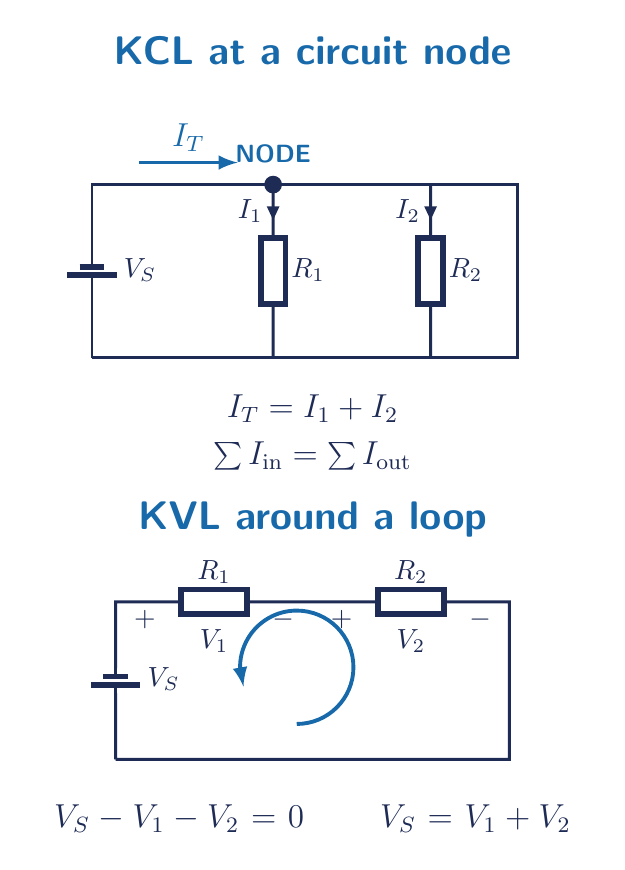
\begin{tikzpicture}[line width=1.05pt,draw=TEJNavy,text=TEJNavy,>=latex]
  \ctikzset{bipoles/length=1.05cm}

  \node[font=\bfseries\Large,text=TEJBlue] at (3.2,7.7) {KCL at a circuit node};
  \coordinate (N) at (2.7,6.0);
  \draw
    (0.4,3.8) to[battery1,l_=$V_S$] (0.4,6.0)
    -- (N) -- (5.8,6.0)
    -- (5.8,3.8) -- (0.4,3.8);
  \draw (N) to[R,l=$R_1$,i>_=$I_1$] (2.7,3.8);
  \draw (4.7,6.0) to[R,l=$R_2$,i>_=$I_2$] (4.7,3.8);
  \draw[->,TEJBlue,line width=1.35pt] (1.0,6.28) -- (2.25,6.28)
    node[midway,above,font=\large] {$I_T$};
  \fill[TEJNavy] (N) circle (3.2pt);
  \node[font=\bfseries\small,text=TEJBlue,above=4pt] at (N) {NODE};
  \node[font=\large] at (3.2,3.15) {$I_T=I_1+I_2$};
  \node[font=\large] at (3.2,2.55) {$\sum I_{\mathrm{in}}=\sum I_{\mathrm{out}}$};

  \node[font=\bfseries\Large,text=TEJBlue] at (3.2,1.75) {KVL around a loop};
  \draw
    (0.7,-1.3) to[battery1,l_=$V_S$] (0.7,0.7)
    to[R,l^=$R_1$,v_>=$V_1$] (3.2,0.7)
    to[R,l^=$R_2$,v_>=$V_2$] (5.7,0.7)
    -- (5.7,-1.3) -- (0.7,-1.3);
  \draw[->,TEJBlue,line width=1.4pt] (3.0,-0.85) arc[start angle=-90,end angle=200,radius=0.72cm];
  \node[font=\large,align=center,text width=7.0cm] at (3.2,-2.05)
    {$V_S-V_1-V_2=0$ \qquad $V_S=V_1+V_2$};
\end{tikzpicture}
\end{document}
